\documentclass[journal,12pt,twocolumn]{IEEEtran}
%
\usepackage{setspace}
\usepackage{gensymb}
%\doublespacing
\singlespacing

%\usepackage{graphicx}
%\usepackage{amssymb}
%\usepackage{relsize}
\usepackage[cmex10]{amsmath}
%\usepackage{amsthm}
%\interdisplaylinepenalty=2500
%\savesymbol{iint}
%\usepackage{txfonts}
%\restoresymbol{TXF}{iint}
%\usepackage{wasysym}
\usepackage{amsthm}
%\usepackage{iithtlc}
\usepackage{mathrsfs}
\usepackage{txfonts}
\usepackage{stfloats}
\usepackage{bm}
\usepackage{cite}
\usepackage{cases}
\usepackage{subfig}
%\usepackage{xtab}
\usepackage{longtable}
\usepackage{multirow}
%\usepackage{algorithm}
%\usepackage{algpseudocode}
\usepackage{enumitem}
\usepackage{mathtools}
\usepackage{steinmetz}
\usepackage{tikz}
\usepackage{circuitikz}
\usepackage{verbatim}
\usepackage{tfrupee}
\usepackage[breaklinks=true]{hyperref}
%\usepackage{stmaryrd}
\usepackage{tkz-euclide} % loads  TikZ and tkz-base
%\usetkzobj{all}
\usetikzlibrary{calc,math}
\usepackage{listings}
    \usepackage{color}                                            %%
    \usepackage{array}                                            %%
    \usepackage{longtable}                                        %%
    \usepackage{calc}                                             %%
    \usepackage{multirow}                                         %%
    \usepackage{hhline}                                           %%
    \usepackage{ifthen}                                           %%
  %optionally (for landscape tables embedded in another document): %%
    \usepackage{lscape}     
\usepackage{multicol}
\usepackage{chngcntr}
%\usepackage{enumerate}

%\usepackage{wasysym}
%\newcounter{MYtempeqncnt}
\DeclareMathOperator*{\Res}{Res}
%\renewcommand{\baselinestretch}{2}
\renewcommand\thesection{\arabic{section}}
\renewcommand\thesubsection{\thesection.\arabic{subsection}}
\renewcommand\thesubsubsection{\thesubsection.\arabic{subsubsection}}

\renewcommand\thesectiondis{\arabic{section}}
\renewcommand\thesubsectiondis{\thesectiondis.\arabic{subsection}}
\renewcommand\thesubsubsectiondis{\thesubsectiondis.\arabic{subsubsection}}

% correct bad hyphenation here
\hyphenation{op-tical net-works semi-conduc-tor}
\def\inputGnumericTable{}                                 %%

\lstset{
%language=C,
frame=single, 
breaklines=true,
columns=fullflexible
}
%\lstset{
%language=tex,
%frame=single, 
%breaklines=true
%}

\begin{document}
%


\newtheorem{theorem}{Theorem}[section]
\newtheorem{problem}{Problem}
\newtheorem{proposition}{Proposition}[section]
\newtheorem{lemma}{Lemma}[section]
\newtheorem{corollary}[theorem]{Corollary}
\newtheorem{example}{Example}[section]
\newtheorem{definition}[problem]{Definition}
%\newtheorem{thm}{Theorem}[section] 
%\newtheorem{defn}[thm]{Definition}
%\newtheorem{algorithm}{Algorithm}[section]
%\newtheorem{cor}{Corollary}
\newcommand{\BEQA}{\begin{eqnarray}}
\newcommand{\EEQA}{\end{eqnarray}}
\newcommand{\define}{\stackrel{\triangle}{=}}
\bibliographystyle{IEEEtran}
%\bibliographystyle{ieeetr}
\providecommand{\mbf}{\mathbf}
\providecommand{\pr}[1]{\ensuremath{\Pr\left(#1\right)}}
\providecommand{\qfunc}[1]{\ensuremath{Q\left(#1\right)}}
\providecommand{\sbrak}[1]{\ensuremath{{}\left[#1\right]}}
\providecommand{\lsbrak}[1]{\ensuremath{{}\left[#1\right.}}
\providecommand{\rsbrak}[1]{\ensuremath{{}\left.#1\right]}}
\providecommand{\brak}[1]{\ensuremath{\left(#1\right)}}
\providecommand{\lbrak}[1]{\ensuremath{\left(#1\right.}}
\providecommand{\rbrak}[1]{\ensuremath{\left.#1\right)}}
\providecommand{\cbrak}[1]{\ensuremath{\left\{#1\right\}}}
\providecommand{\lcbrak}[1]{\ensuremath{\left\{#1\right.}}
\providecommand{\rcbrak}[1]{\ensuremath{\left.#1\right\}}}
\theoremstyle{remark}
\newtheorem{rem}{Remark}
\newcommand{\sgn}{\mathop{\mathrm{sgn}}}
\providecommand{\abs}[1]{\left\vert#1\right\vert}
\providecommand{\res}[1]{\Res\displaylimits_{#1}} 
\providecommand{\norm}[1]{\left\lVert#1\right\rVert}
%\providecommand{\norm}[1]{\lVert#1\rVert}
\providecommand{\mtx}[1]{\mathbf{#1}}
\providecommand{\mean}[1]{E\left[ #1 \right]}
\providecommand{\fourier}{\overset{\mathcal{F}}{ \rightleftharpoons}}
%\providecommand{\hilbert}{\overset{\mathcal{H}}{ \rightleftharpoons}}
\providecommand{\system}{\overset{\mathcal{H}}{ \longleftrightarrow}}
	%\newcommand{\solution}[2]{\vec{Solution:}{#1}}
\newcommand{\solution}{\noindent \vec{Solution: }}
\newcommand{\cosec}{\,\text{cosec}\,}
\providecommand{\dec}[2]{\ensuremath{\overset{#1}{\underset{#2}{\gtrless}}}}
\newcommand{\myvec}[1]{\ensuremath{\begin{pmatrix}#1\end{pmatrix}}}
\newcommand{\mydet}[1]{\ensuremath{\begin{vmatrix}#1\end{vmatrix}}}
%\numberwithin{equation}{section}
\numberwithin{equation}{subsection}
%\numberwithin{problem}{section}
%\numberwithin{definition}{section}
\makeatletter
\@addtoreset{figure}{problem}
\makeatother
\let\StandardTheFigure\thefigure
\let\vec\mathbf
%\renewcommand{\thefigure}{\theproblem.\arabic{figure}}
\renewcommand{\thefigure}{\theproblem}
%\setlist[enumerate,1]{before=\renewcommand\theequation{\theenumi.\arabic{equation}}
%\counterwithin{equation}{enumi}
%\renewcommand{\theequation}{\arabic{subsection}.\arabic{equation}}
\def\putbox#1#2#3{\makebox[0in][l]{\makebox[#1][l]{}\raisebox{\baselineskip}[0in][0in]{\raisebox{#2}[0in][0in]{#3}}}}
     \def\rightbox#1{\makebox[0in][r]{#1}}
     \def\centbox#1{\makebox[0in]{#1}}
     \def\topbox#1{\raisebox{-\baselineskip}[0in][0in]{#1}}
     \def\midbox#1{\raisebox{-0.5\baselineskip}[0in][0in]{#1}}
\vspace{3cm}
\title{ASSIGNMENT 4}
\author{YENIGALLA SAMYUKTHA\\EE20MTECH14019}
%
\maketitle
\newpage
%\tableofcontents
\bigskip
\renewcommand{\thefigure}{\theenumi}
\renewcommand{\thetable}{\theenumi}
%
\begin{abstract}
This document finds the equation of circle passing through three given points.
\end{abstract}
Download all python codes from 
%
\begin{lstlisting}
https://github.com/EE20MTECH14019/EE5609/tree/master/Assignment_4/Codes
\end{lstlisting}
%
and latex-tikz codes from 
%
\begin{lstlisting}
https://github.com/EE20MTECH14019/EE5609/tree/master/Assignment_4
\end{lstlisting}
%
\section{Problem}
\item Find the equation of the circle that passes through the points $\myvec{2\\3},\myvec{3\\2},\myvec{5\\1}$
\section{Solution}
\item The general equation of circle is represented as
\begin{align}
    \label{circleeq}
    \vec{x}^T\vec{x}-2\vec{c}^T\vec{x}+f=0
\end{align}
where $\vec{c}$ is the center of the circle. Substituting the given points in the equation \eqref{circleeq}, we obtain
\begin{align}
    \label{points}
    2\myvec{2&3}\vec{c}-f=13\\
    2\myvec{3&2}\vec{c}-f=13\\
    2\myvec{5&1}\vec{c}-f=36
\end{align}
can be expressed in matrix form as 
\begin{align}
    \label{matrix}
    \myvec{4&6&-1\\6&4&-1\\10&2&-1}\myvec{\vec{c}\\f}=\myvec{13\\13\\26}
\end{align}
\begin{figure}[!ht]
\centering
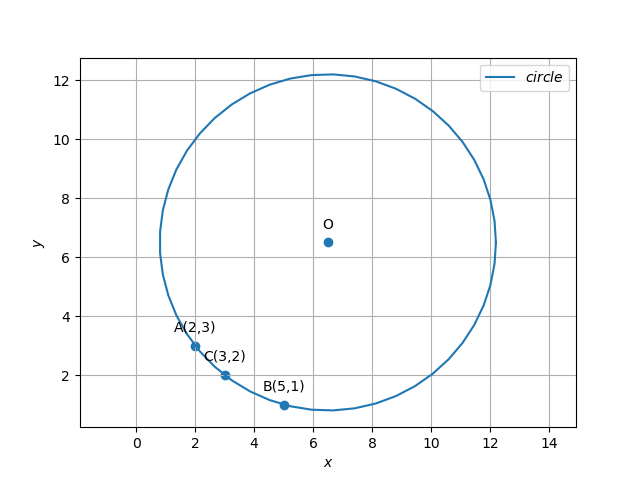
\includegraphics[width=\columnwidth]{Circle.png}
\caption{Circle passing through the points A,B,C with center O}
\label{fig1}
\end{figure}
The augmented matrix for \eqref{matrix} can be row reduced as follows
\begin{align}
    \myvec{4&6&-1&13\\6&4&-1&13\\10&2&-1&26}\\
    \xleftrightarrow[R_2\leftarrow4R_2-6R_1]{R_3\leftarrow 4R_3-10R_1}
    \myvec{4&6&-1&13\\0&-20&2&-26\\0&-52&6&-26}\\
    \xleftrightarrow[]{R_3\leftarrow 5R_3-13R_2}
    \myvec{4&6&-1&13\\0&-20&2&-26\\0&0&4&208}\\
    \xleftrightarrow[R_1\leftarrow 4R_1+R_3]{R_2\leftarrow 2R_2-R_3}
   \myvec{16&24&0&260\\0&-40&0&-260\\0&0&4&208}\\
   \xleftrightarrow[]{R_1\leftarrow 5R_1+3R_2}
   \myvec{80&0&0&520\\0&-40&0&-260\\0&0&4&208}\\
   \label{red}
   \xleftrightarrow[R_1\leftarrow \frac{R_1}{40}]{R_2\leftarrow\frac{R_2}{-20},R_3\leftarrow\frac{R_3}{4}}
   \myvec{2&0&0&13\\0&2&0&13\\0&0&1&52}
\end{align}
From the matrix \eqref{red},
\begin{align}
    \vec{c}=\myvec{\frac{13}{2}\\\frac{13}{2}}\\
    k=52\\
    r=\sqrt{\norm{\vec{c}}^2-f}=11
\end{align}
Hence the circle equation can be written as,
\begin{align}
    \vec{x}^T\vec{x}-2\myvec{\frac{13}{2}&\frac{13}{2}}^T\vec{x}+52=0
\end{align}
\end{document}
